\chapter{Eredmények}
\pagestyle{headings}


\section{Sejtekből kiszabaduló káliumion koncentráció közelítő számítása}

\emph{Candida albicans} sejttérfogat \cite{chaffin1984relationship}

10$^7$ sejt/ml $\cdot$ 10 ml = 10$^8$ sejt

10$^8$ sejt $\cdot$ 20 $\upmu m^3$/sejt = 2 $\cdot$ 10$^9$ $\upmu m^3$ = 2 $\cdot$ 10$^{-6}$ $dm^3$

ha az összes sejt szétesik, és az összes intracelluláris káliumion kiszabadul az extracelluláris térbe:

2 $\cdot$ 10$^{-6}$ $dm^3$ $\cdot$ 0.1 M = 2 $\cdot$ 10$^{-7}$ mol

2 $\cdot$ 10$^{-7}$ mol / 0.01 $dm^3$ = 2 $\cdot$ 10$^{-5}$ M

\section{Káliumion szelektív elektródok kalibrációja}

\section{Káliumion kiáramlás nyomon követése ionszelektív elektróddal}

\begin{figure}
\centering
\includegraphics[width=0.7\textwidth, angle=-90]{img/meres.eps}
\caption{képaláírás}
\label{fig:mérések}
\end{figure}

Ahogy az a \ref{fig:mérések}. ábrán látható.


